\documentclass[11pt]{article}

\usepackage{amsmath, amsthm, amssymb, amsfonts}
\usepackage{thmtools}
\usepackage{graphicx}
\usepackage{setspace}
\usepackage{geometry}
\usepackage{float}
\usepackage{hyperref}
\usepackage[utf8]{inputenc}
\usepackage[english]{babel}
\usepackage{framed}
\usepackage[dvipsnames]{xcolor}
\usepackage{tcolorbox}
\usepackage{xcolor}
\usepackage{color}
\usepackage{listings}

\DeclareFixedFont{\ttb}{T1}{txtt}{bx}{n}{12}
\DeclareFixedFont{\ttm}{T1}{txtt}{m}{n}{12}

\definecolor{deepblue}{rgb}{0,0,0.5}
\definecolor{deepred}{rgb}{0.6,0,0}
\definecolor{deepgreen}{rgb}{0,0.5,0}

\definecolor{solarized@base03}{HTML}{002B36}
\definecolor{solarized@base02}{HTML}{073642}
\definecolor{solarized@base01}{HTML}{586e75}
\definecolor{solarized@base00}{HTML}{657b83}
\definecolor{solarized@base0}{HTML}{839496}
\definecolor{solarized@base1}{HTML}{93a1a1}
\definecolor{solarized@base2}{HTML}{EEE8D5}
\definecolor{solarized@base3}{HTML}{FDF6E3}
\definecolor{solarized@yellow}{HTML}{B58900}
\definecolor{solarized@orange}{HTML}{CB4B16}
\definecolor{solarized@red}{HTML}{DC322F}
\definecolor{solarized@magenta}{HTML}{D33682}
\definecolor{solarized@violet}{HTML}{6C71C4}
\definecolor{solarized@blue}{HTML}{268BD2}
\definecolor{solarized@cyan}{HTML}{2AA198}
\definecolor{solarized@green}{HTML}{859900}

\hypersetup { colorlinks, linkcolor=Black, urlcolor=solarized@blue}

\lstset{language=C++,
    basicstyle=\footnotesize\ttfamily,
    numbers=left,
    numberstyle=\footnotesize,
    tabsize=2,
    breaklines=true,
    escapeinside={@}{@},
    numberstyle=\tiny\color{solarized@base01},
    keywordstyle=\color{solarized@green},
    stringstyle=\color{solarized@cyan}\ttfamily,
    identifierstyle=\color{solarized@blue},
    commentstyle=\color{solarized@base01},
    emphstyle=\color{solarized@red},
    frame=single,
    rulecolor=\color{solarized@base2},
    rulesepcolor=\color{solarized@base2},
    showstringspaces=false
}


\colorlet{LightGreen}{Green!15}

\newcommand{\HRule}[1]{\rule{\linewidth}{#1}}

\declaretheoremstyle[name=Solution,]{thmsty}
\declaretheorem[style=thmsty,numberwithin=section]{solution}
\tcolorboxenvironment{solution}{colback=LightGreen}


\setstretch{1.2}
\geometry{
    textheight=9in,
    textwidth=5.5in,
    top=1in,
    headheight=12pt,
    headsep=25pt,
    footskip=30pt
}

% ------------------------------------------------------------------------------

\begin{document}
	
\pagenumbering{gobble}


\title{ \normalsize \textsc{}
    \\ [2.0cm]
    \HRule{1.5pt} \\
    \LARGE \textbf{\uppercase{Binary Search Trees}
        \HRule{2.0pt} \\ [0.6cm] \LARGE{CSE 4303 \\  Data Structures} \vspace*{10\baselineskip}}
}
\date{\today}
\author{\textbf{Hasin Mahtab} \\ 
    210042174 \\
    Department of CSE \\
    B.Sc in Software Engineering}

\maketitle
\newpage

\tableofcontents
\newpage
\pagenumbering{arabic}
% ------------------------------------------------------------------------------

\section{Detecting Financial Anomalies}
Financial experts are working with a cutting-edge stock trading system to uncover probable anomalies in the trading behaviour of specific equities. You are entrusted with creating a function that can recognise triplets of stock trades within a Binary Search Tree (BST) whose total transaction amounts add up to a particular target sum to assist them. The stock trading system maintains a BST of stock trades, where each trade is represented as a node with the following information:
\begin{itemize}
    \item \textbf{Trade ID:} A unique identifier for each trade.
    \item \textbf{Stock Symbol:} The symbol of the traded stock.
    \item \textbf{Transaction Amount:} The monetary value of the trade.
\end{itemize}

The financial analysts suspect that certain patterns of three trades (triplets) with a specific total transaction amount might indicate irregular trading behavior.

    \subsection{Input}
    \begin{itemize}
        \item \textbf{root:} Root of a Binary Search Tree (1 $\leq$ (nodes in the BST) $\leq$ $10^5$).
        \item \textbf{targetSum:} For which triplets need to be found (0.0 $\leq$ targetSum $\leq$ 1e9).
    \end{itemize}
    

    \subsection{Output}
    \begin{itemize}
        \item A list of triplets (lists) containing stock symbols whose total transaction amounts add up to the target sum.
    \end{itemize}
    \subsection{Example}
    \begin{lstlisting}
TradeNode* tradeTree = new TradeNode("A1", "AAPL", 100.0);
tradeTree->left = new TradeNode("A2", "GOOGL", 150.0);
tradeTree->right = new TradeNode("A3", "AMZN", 200.0);
tradeTree->left->left = new TradeNode("A4", "AAPL", 50.0);
tradeTree->left->right = new TradeNode("A5", "GOOGL", 120.0);
tradeTree->right->left = new TradeNode("A6", "AAPL", 180.0);
tradeTree->right->right = new TradeNode("A7", "MSFT", 300.0);

double targetSum = 500.0;
\end{lstlisting}
The expected \textbf{output} for this example would be:
\begin{lstlisting}
Triplets with target sum 500:
[AAPL GOOGL MSFT ]
[AAPL AMZN MSFT ]
\end{lstlisting}
\subsubsection{Explanation}
\begin{itemize}
    \item The first triplet [AAPL, GOOGL, MSFT] consists of trades with transaction amounts 100.0, 120.0, and 300.0, which sum up to the target sum of 500.0.
    \item The second triplet [AAPL, AMZN, MSFT] consists of trades with transaction amounts 50.0, 200.0, and 300.0, which also sum up to the target sum of 500.0.
\end{itemize}


% ------------------------------------------------------------------------------
% ------------------------------------------------------------------------------

\section{Binary Search Tree}
    \subsection{Introduction}
    A binary search tree is either an empty data structure represented by nullptr or a single node x, whose left subtree is a BST of smaller values than x and whose right subtree is a BST of larger values than x. This special property called the BST-property, which is given as follows:
    
    \begin{itemize}
        \item For all nodes x and y, if y belongs to the left subtree of x, then the key at y is less than the key at x, and if y belongs to the right subtree of x, then the key at y is greater than the key at x.
    \end{itemize}
    
    \begin{figure}[htbp]
        \center
        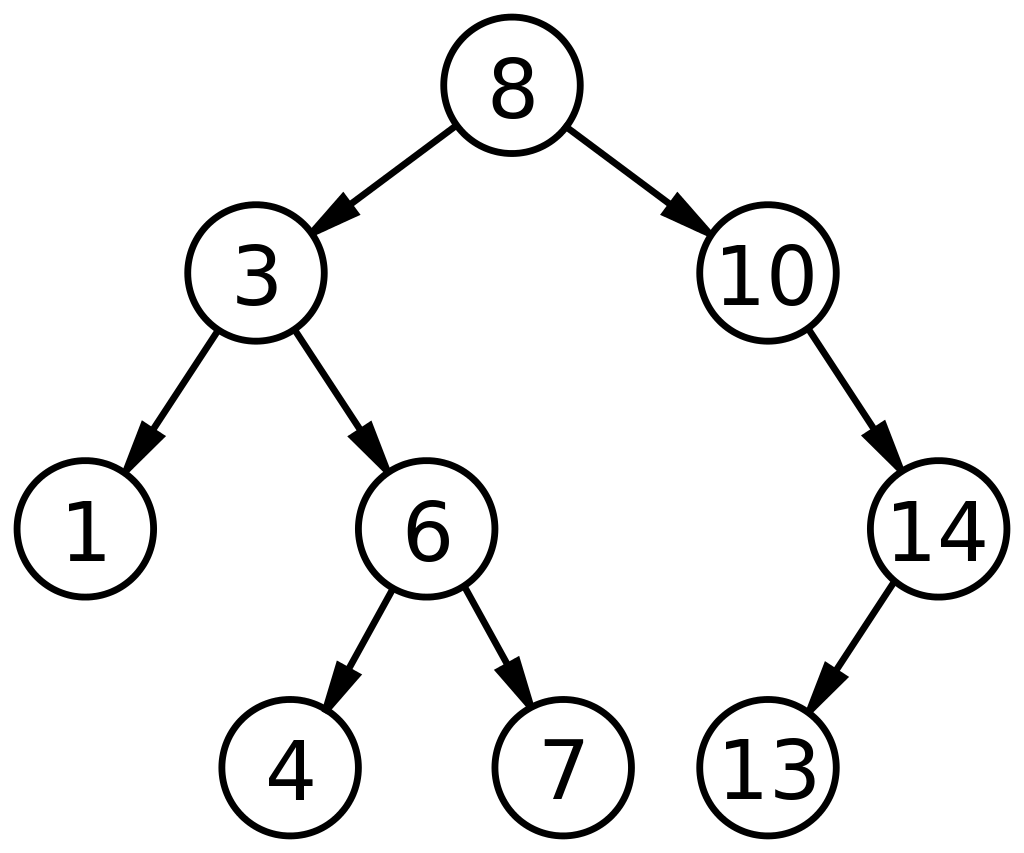
\includegraphics[scale=0.2]{bstexample.png}
        \caption{A simple binary search tree}
    \end{figure}
    
    In the Binary search tree, The values in the left subtree are all smaller than the root 8, whereas the values in the right subtree are all greater. Each node has the following attributes:
    \begin{itemize}
        \item p, left, and right, which are pointers to the
    parent, the left child, and the right child,
    respectively.
    \item key, which is key stored at the node.
    \end{itemize}

    \subsection{Successor and predecessor}
    For certain operations, given a node x , finding the successor or predecessor of x is crucial. Assuming all the keys of the BST are distinct, the successor of a node x in BST is the node with the smallest key greater than x 's key. On the other hand, the predecessor of a node x in BST is the node with the largest key smaller than x 's key. Following is pseudocode for finding the successor and predecessor of a node x in BST.
    
    \subsection{Operations}
    Binary search trees allow binary search for fast lookup, addition, and removal of data items. Since the nodes in a BST are laid out so that each comparison skips about half of the remaining tree, the lookup performance is proportional to that of binary logarithm.

        \subsubsection{Traversal}
        We define "traversal" as visiting all nodes in a graph. The ordering of the three items to visit: the current node, the left subtree, and the right subtree, can be used to specify traversal methods. Then there are three options.

        \begin{itemize}
            \item Inorder : Left Subtree $\rightarrow$ Parent Node $\rightarrow$ Right Subtree
            \item Preorder : Parent Node $\rightarrow$ Left Subtree $\rightarrow$ Right Subtree
            \item Postorder : Left Subtree $\rightarrow$ Right Subtree $\rightarrow$ Parent Node
        \end{itemize}

        \subsubsection{Insertion}
        By retaining the binary search tree's property, a new key is always put at the leaf. We begin our search for a key at the root and go until we reach a leaf node. When a leaf node is discovered, the new node is inserted as a child of that node.\newline

        When looking for a place to insert a new key, traverse the tree from root to leaf, comparing keys stored in the tree's nodes and selecting whether to continue searching in the left or right subtrees based on the comparison. In other words, we evaluate the root and recursively insert the new node to the left subtree if its key is less than the root's key or to the right subtree if its key is larger than or equal to the root's key.\newline
        
Following is the Insert function implementation of the above approach in C++
\begin{lstlisting}
Node* insert(Node* root, int key)
{
    // if the root is null, create a new node and return it
    if (root == nullptr) {
        return new Node(key);
    }
 
    // if the given key is less than the root node, recur for the left subtree
    if (key < root->data) {
        root->left = insert(root->left, key);
    }
    // if the given key is more than the root node, recur for the right subtree
    else {
        root->right = insert(root->right, key);
    }
 
    return root;
}
\end{lstlisting}

        \begin{figure}[H]
            \centering
            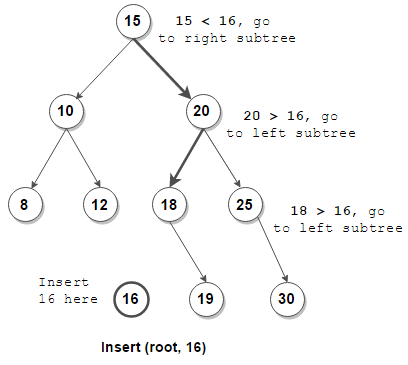
\includegraphics[scale=0.7]{InsertBST.png}
            \caption{Inserting 16 in BST tree}\label{InsertBST}
        \end{figure}
    
        \subsubsection{Searching}
        Searching for a given key in a binary search tree can be done recursively or iteratively.\newline
        
        The search begins with an examination of the root node. The key being searched for does not exist in the tree if the tree is null. Otherwise, the search is successful and the node is returned if the key matches that of the root. If the key is smaller than the root, the search advances to the left subtree. Similarly, if the key is greater than the root, the search moves on to the appropriate subtree. This process is done until either the key or the remaining subtree is located.\newline

Following is the Search function implementation of the above approach in C++
\begin{lstlisting}
void search(Node* root, int key, Node* parent)
{
    // if the key is not present in the key
    if (root == nullptr)
    {
        cout << "Key not found";
        return;
    }
 
    // if the key is found
    if (root->data == key)
    {
        if (parent == nullptr) {
            cout << "The node with key " << key << " is root node";
        }
        else if (key < parent->data)
        {
            cout << "The given key is the left node of the node with key "
                 << parent->data;
        }
        else  {
            cout << "The given key is the right node of the node with key "
                 << parent->data;
        }
 
        return;
    }
\end{lstlisting}

        \begin{figure}[H]
            \centering
            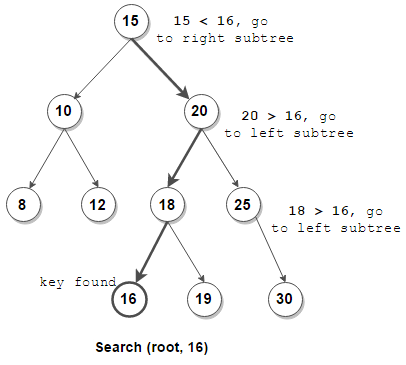
\includegraphics[scale=0.7]{BSTSearch.png}
            \caption{Searching 16 in BST tree}\label{BSTSearch}
        \end{figure}
        
        
        \subsubsection{Deletion}
        Given a BST, the task is to delete a node in this BST, which can be broken down into 3 scenarios:
        \begin{itemize}
            \item \textbf{Deleting a node with no children:} Remove the node from the tree.
        \begin{figure}[H]
            \centering
            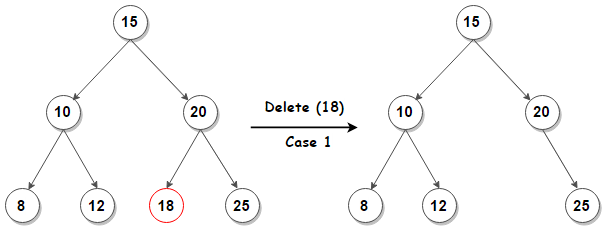
\includegraphics[scale=0.7]{DeletionBSTC1.png}
            \caption{Searching 16 in BST tree}\label{DeletionBSTC1}
        \end{figure}

            \item \textbf{Deleting a node with two children:} Call the node to be deleted N. Do not delete N. Instead, choose either its inorder successor node or its inorder predecessor node, R. Copy the value of R to N, then recursively call delete on R until reaching one of the first two cases. If we choose the inorder successor of a node, as the right subtree is not NULL (our present case is a node with 2 children), then its inorder successor is a node with the least value in its right subtree, which will have at a maximum of 1 subtree, so deleting it would fall in one of the first 2 cases.

        \begin{figure}[H]
            \centering
            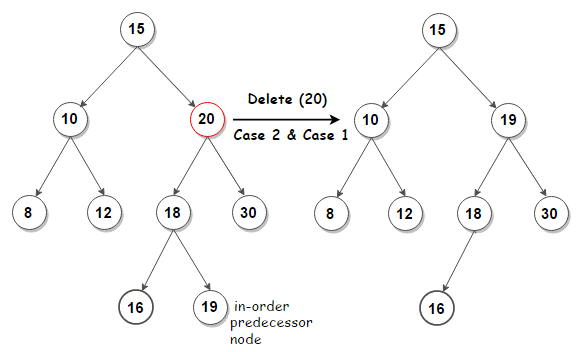
\includegraphics[scale=0.7]{DeletionBSTC2.png}
            \caption{Searching 16 in BST tree}\label{DeletionBSTC2}
        \end{figure}

            \item \textbf{Deleting a node with one child:} Remove the node and replace it with its child.

            \begin{figure}[H]
            \centering
            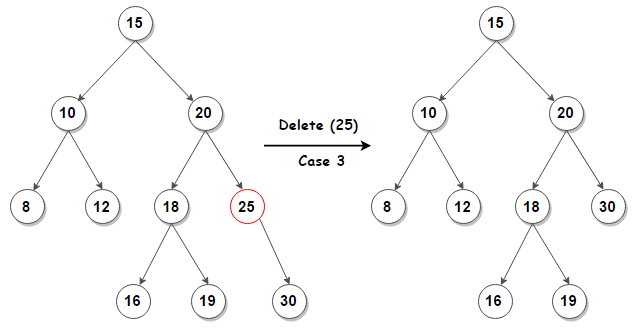
\includegraphics[scale=0.7]{DeletionBSTC3.png}
            \caption{Searching 16 in BST tree}\label{DeletionBSTC3}
        \end{figure}
        \end{itemize}

        Nodes with children are harder to delete. As with all binary trees, a node’s inorder successor is its right subtree’s leftmost child, and a node’s inorder predecessor is the left subtree’s rightmost child. In either case, this node will have zero or one child. Delete it according to one of the two simpler cases above.

% ------------------------------------------------------------------------------
% ------------------------------------------------------------------------------
	
\section{Problem Analysis}
We are provided a Binary Search Tree (BST) representing stock trades in this case. In the BST, each trade is represented as a node, with information such as the trade ID, stock symbol, and transaction amount. The purpose is to find triplets of stock trades whose total transaction values add up to a certain amount.
    \subsection{Intuition behind the solution}
    \subsubsection{BST Traversal}
We need to traverse the given BST to explore all possible triplets. The traversal can be done using a recursive approach, visiting each node in a depth-first manner.

\subsubsection{Triplet Detection}
\begin{itemize}
    \item While traversing the BST, we keep track of the current triplet and a set of visited stock symbols within the current triplet.
    \item When a node is visited, we check if its stock symbol is already in the set of visited symbols. If it is, we remove it from the set (backtracking).
    \item We also check if the current triplet is complete. If it is, we calculate the sum of transaction amounts and check if it equals the target sum.
    \item If a valid triplet is found, it is added to the result.
\end{itemize}

\subsubsection{Backtracking}
Backtracking is essential to explore all possible combinations of triplets and to ensure that the set of visited symbols is appropriately updated.

    \subsection{Solution steps}
    To solve the problems, let's go step by step -
    \begin{enumerate}
        \item Initialize an empty set visitedStocks
        \item Initialize an empty list currentTriplet
        \item Initialize an empty list result
        \item Start the recursive detection process
        \item return result
    \end{enumerate}

    A simple solution for the process is as follows: 

    \begin{lstlisting}
#include <iostream>
#include <vector>
using namespace std;

struct TradeNode
{
    string tradeId;
    string stockSymbol;
    double transactionAmount;
    TradeNode *left;
    TradeNode *right;

    TradeNode(string id, string symbol, double amount)
        : tradeId(id), stockSymbol(symbol), transactionAmount(amount), left(nullptr), right(nullptr) {}
};

void detectAnomaliesInStockTrades(TradeNode *root, double targetSum, vector<string> &currentTriplet, vector<vector<string>> &result)
{
    if (!root)
    {
        return;
    }

    // Check if the current triplet is complete
    if (currentTriplet.size() < 3)
    {
        // Add the stock symbol to the current triplet
        currentTriplet.push_back(root->stockSymbol);
    }
    else
    {
        double tripletSum = 0.0;
        for (const string &symbol : currentTriplet)
        {
            tripletSum += root->transactionAmount;
        }

        if (tripletSum == targetSum)
        {
            // Add the current triplet to the result
            result.push_back(currentTriplet);
        }
    }

    detectAnomaliesInStockTrades(root->left, targetSum, currentTriplet, result);
    detectAnomaliesInStockTrades(root->right, targetSum, currentTriplet, result);

    currentTriplet.pop_back();
}

vector<vector<string>> findTripletsInBST(TradeNode *root, double targetSum)
{
    vector<string> currentTriplet;
    vector<vector<string>> result;

    detectAnomaliesInStockTrades(root, targetSum, currentTriplet, result);
    return result;
}

int main()
{
    TradeNode *tradeTree = new TradeNode("A1", "AAPL", 100.0);
    tradeTree->left = new TradeNode("A2", "GOOGL", 150.0);
    tradeTree->right = new TradeNode("A3", "AMZN", 200.0);
    tradeTree->left->left = new TradeNode("A4", "AAPL", 50.0);
    tradeTree->left->right = new TradeNode("A5", "GOOGL", 120.0);
    tradeTree->right->left = new TradeNode("A6", "AAPL", 180.0);
    tradeTree->right->right = new TradeNode("A7", "MSFT", 300.0);

    double targetSum = 500.0;

    vector<vector<string>> anomalies = findTripletsInBST(tradeTree, targetSum);

    cout << "Triplets with target sum " << targetSum << ":" << endl;
    for (const vector<string> &triplet : anomalies)
    {
        cout << "[";
        for (const string &symbol : triplet)
        {
            cout << symbol << " ";
        }
        cout << "]" << endl;
    }

    return 0;
}
\end{lstlisting}
    
    \subsection{Complexity Analysis}
    \subsubsection{Time Complexity}
    The time complexity of the solution depends on the number of nodes in the Binary Search Tree (BST) and the number of valid triplets that satisfy the conditions.

    \begin{itemize}
        \item \textbf{Traversal Time:} The depth-first traversal of the BST contributes to the time complexity. In the worst case, we may need to visit all nodes in the BST. \textbf{O(N)}, where N is the number of nodes in the BST.
        \item \textbf{Triplet Detection Time:} Checking and detecting triplets involves constant time operations (e.g., updating sets, checking target sum). \textbf{O(1)} per node.
        \item \textbf{Backtracking:} Backtracking is performed when a stock symbol is revisited within a triplet. The set of visited symbols is updated. \textbf{O(1)} per backtracking step.
    \end{itemize}
    
    \subsubsection{Space Complexity}
    The space complexity of the solution is influenced by the memory required for recursive calls, the storage of visited symbols, and the depth of the recursion stack.

    \begin{itemize}
        \item \textbf{Recursive Call Stack:} The space required for the recursive call stack depends on the height of the BST. In the worst case, the tree is skewed, leading to a height of N. \textbf{O(N)}, where N is the height of the BST.
        \item \textbf{Visited Symbols Set:} The set of visited symbols stores distinct stock symbols within a triplet. \textbf{O(1)} per node (constant number of symbols).
        \item \textbf{Current Triplet Storage:} The current triplet vector stores stock symbols temporarily during the recursive exploration. \textbf{O(1)} per node (constant number of symbols).
        \item \textbf{Auxiliary Variables:} Additional auxiliary variables and function parameters contribute to constant space usage. \textbf{O(1)}.
    \end{itemize}


% ------------------------------------------------------------------------------
% ------------------------------------------------------------------------------

\section{Applications of BST}
    Due to the BST property, BSTs allow for efficient searching by repeatedly dividing the search space in half, which makes it an important data structure in computer science and many other fields.
    \subsection{Efficient to use BST}
    \begin{itemize}
        \item A BST can be used to sort a large dataset. By inserting the elements of the dataset into a BST and then performing an in-order traversal, the elements will be returned in sorted order.

        \item BSTs are used to implement Huffman coding algorithm. While binary trees are involved in the Huffman coding algorithm, they are not necessarily implemented as BSTs.

        \item BSTs can be used to implement symbol tables, which are used to store data such as variable and function names in a programming language. 

        \item In the case of databases, an index is often implemented as a data structure that maps the values of one or more columns to the corresponding records in the database table. A Binary Search Tree is a type of data structure that is well-suited for this purpose.
    \end{itemize}
    \subsection{Inefficient to use BST}
    \begin{itemize}
        \item They are not well-suited for data structures that need to be accessed randomly, since the time complexity for search, insert, and delete operations is O(log n), which is good for large data sets, but not as fast as some other data structures such as arrays or hash tables.

        \item A BST can be imbalanced or degenerated which can increase the complexity.

        \item They are not guaranteed to be balanced, which means that in the worst case, the height of the tree could be O(n) and the time complexity for operations could degrade to O(n). 
    \end{itemize}


% ------------------------------------------------------------------------------
% ------------------------------------------------------------------------------
        
\section{Practice Problems}
    Some practice problems to apply the knowledge from this article.
    \subsection{Binary Search Tree}
    Given a binary tree, your task is to choose a maximal set S of connected nodes in the given tree so that these nodes and the relations (left child, right child, or ancestor) among them form a binary search tree.
    \href{https://codeforces.com/problemset/gymProblem/100499/E}{Codeforces 100499E}
    \subsection{Broken BST}
    A rooted binary tree where each vertex has at most two children. The tree has one vertex that doesn't have a parent, which is the root. Each vertex has an integer number written on it.
    \href{https://codeforces.com/problemset/problem/797/D}{Codeforces 797D}
    \subsection{Monk and his Friends}
    Monk is standing at the door of his classroom. There are currently N students in the class, i'th student got Ai candies. There are still M more students to come. At every instant, a student enters the class and wishes to be seated with a student who has exactly the same number of candies. For each student, Monk shouts YES if such a student is found, NO otherwise.
    \href{https://www.hackerearth.com/practice/data-structures/trees/binary-search-tree/practice-problems/algorithm/monk-and-his-friends/}{Monk and his Friends}

% ------------------------------------------------------------------------------
% ------------------------------------------------------------------------------

\bibliographystyle{IEEEtran}
\bibliography{References.bib}


\begin{itemize}
    \item \href{https://en.wikipedia.org/wiki/Binary_search_tree}{Binary Search Tree - Wikipedia}

    \item \href{https://www.cs.rochester.edu/u/gildea/csc282/slides/C12-bst.pdf}{C12 - BST, University of Rochester}

    \item \href{https://www.geeksforgeeks.org/binary-search-tree-data-structure/}{Binary Search Tree - GeeksforGeeks}

    \item \href{https://www.techiedelight.com/}{Operations in BST}

    \item \href{https://codeforces.com/}{Practice: Binary Search Trees}

    \item \href{https://www.techiedelight.com/find-triplet-with-given-sum-bst/}{Find a triplet with the given sum in a BST}

\end{itemize}

 
% ------------------------------------------------------------------------------
% ------------------------------------------------------------------------------
	
\end{document}